In this section we derive the conservation equations using a two-fluid formulation.%the two-fluid formulation of the balance equations. %derive the equations governing the two fluid motion.
While the derivation of this formulation is available in various studies such as those by \citet{kataoka1986local,lhuillier2010multiphase,ishii2010thermo,morel2015mathematical} our approach here enables us to introduce specific notations and key results that will prove useful for later discussions. %Although the derivation of the two fluid model may be found in many other studies \citep{lhuillier,ishii,morel,delhaye} this derivation allows us to present the notations and some results which will be usefull later on. %starting from 
\begin{figure}[h!]
    \centering
    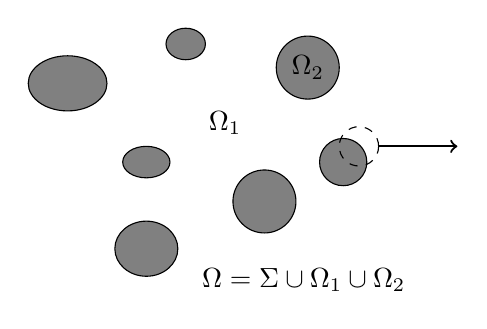
\begin{tikzpicture}
        \foreach \x/\y/\ra/\r in {
        1/3/0.2/0.25,
        2.55/2.7/0.4/0.4,
        0.5/0.4/0.35/0.4,
        2/1/0.4/0.4,
        3/1.5/0.3/0.3,
        0.5/1.5/0.2/0.3,
        -0.5/2.5/0.35/0.5}{
            \draw[fill=gray](\x,\y) ellipse(\r cm and \ra cm);
        }
        \draw[dashed](3.2,1.7)circle(0.25);
        % \draw[thick,->](3.2,1.7)++(0.1767,0.1767)--++(0.4,0.4)--++(1,0);
        \draw[thick,->](3.2,1.7)++(0.25,0)--++(1,0);
        \draw(2.55,2.7)node{$\Omega_2$};
        \draw(1.5,2)node{$\Omega_1$};
        \draw(2.5,0)node{$\Omega = \Sigma \cup \Omega_1 \cup \Omega_2$};
        % \draw(2.5,-1)node{$\Sigma = \sum_\alpha \Sigma_\alpha$};
        % \draw(2.5,-0.5)node{$\Omega_2 = \sum_\alpha \Omega_\alpha$};
    \end{tikzpicture}
    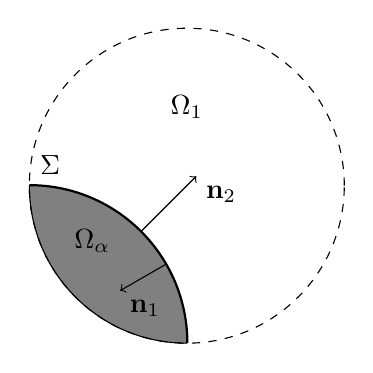
\begin{tikzpicture}%[scale = 0.9]
        \draw[very thick](0:2)arc(0:90:2)node[above right]{$\Sigma$};
        \draw[fill=gray](0:2)arc(0:90:2)arc(180:270:2);
        \draw[dashed](2,2)circle(2);
        \draw[->](1.42,1.42)--++(0.7,0.7)node[below right]{$\textbf{n}_2$};
        \draw[->](1.73,1)--++(-0.577,-0.333)node[below right]{$\textbf{n}_1$};
        \draw(2,3)node{$\Omega_1$};
        \draw(0.8,1.3)node{$\Omega_\alpha$};
    \end{tikzpicture}
    \caption{Topology of dispersed two-phase flows.}%Domain definitions and scheme of the topology of dispersed two-phase flows.}
    \label{fig:Scheme}
\end{figure}

We consider a system consisting of two phases, separated by a sharp interface $\Sigma(t)$ which evolves over time. 
For further insights into the modeling of sharp interface thermodynamics, a comprehensive review may be found in \cite{bothe2022sharp}. 
Each phase subdomain is denoted as $\Omega_1(t)$ and $\Omega_2(t)$, representing the continuous phase (1) and the dispersed phase (2) respectively (refer to Figure \ref{fig:Scheme}).
The entire domain, denoted as $\Omega$, is defined as the union of $\Omega_1$, $\Omega_2$, and $\Sigma$.
To track the position of the phase indexed $k$ and the interfaces, we introduce the phase indicator function $\chi _k$ defined as
\begin{align}
    \chi_k(\textbf{x},t) =  \left\{
      \begin{tabular}{cc}
        $1 \;\text{if} \;\textbf{x} \in \Omega_k(t)$\\
        $0 \;\text{if} \;\textbf{x} \notin \Omega_k(t)$
      \end{tabular}
      \right.
      \text{for $k = 1,2$}.
      \label{eq:PIF}
%    && \delta_I(\textbf{x},t) =  \left\{
%      \begin{tabular}{cc}
%        $1 \;\text{if} \;\textbf{x} \in \Sigma(t)$\\
%        $0 \;\text{if} \;\textbf{x} \notin \Sigma(t)$
%      \end{tabular}
%      \right.,
%       \label{eq:PIF}
\end{align}
To enhance clarity, we will omit the time and position parameters from $\chi_k(\textbf{x},t)$ in the subsequent sections.

\subsection{Topological equations}
Using the distribution formalism, one may show that $\chi_k$ obeys the following relations \citep{drew1983mathematical}. 
\begin{align}
    \pddt \chi_k
    + \textbf{u}_I^0 \cdot \grad \chi_k
    &= 0,
    \label{eq:dt_chi_k}\\
    \label{eq:grad_chi_k}
    \grad \chi_k
    &= - \delta_I \textbf{n}_k. 
\end{align}
where $u^0_I$ is the velocity of the interface and $\delta_I$ is the Dirac function localized on the interface.
Then, to describe the evolution of $\delta_I$ we take the gradient of \ref{eq:dt_chi_k} and the gradient of \ref{eq:grad_chi_k} which yields two equations of the interface indicator function \citep{morel2007surface},
\begin{align}
    \pddt \delta_I
    + \div (\delta_I \textbf{u}_I^0)
    &= \delta_I \divI \textbf{u}_I,
    \label{eq:dt_delta_I}\\
    \grad\delta_I 
    &= \textbf{n} \cdot \grad (\textbf{n} \delta_I),
    \label{eq:grad_delta_I}
\end{align}
where $\divI(\ldots) = (\textbf{I}-\textbf{nn})\cdot \div(\ldots)$ is the surface divergence operator. \ref{eq:dt_chi_k}, \ref{eq:dt_delta_I}, \ref{eq:grad_delta_I} and \ref{eq:grad_chi_k} are commonly referred to as the topological equations as it describe the evolution in space and time of the topology.


\subsection{Local conservation equations}
\label{sec:local_eq}

Let $f_k^0(\textbf{x},t)$ denote a volumetric quantity of arbitrary tensorial order defined in $\Omega_k(t)$.
Likewise, let $f_I^0(\textbf{x}_I,I)$ represent an arbitrary surface property defined on $\Sigma(t)$.
Using the strategy outlined in \citep{bothe2022sharp,morel2015mathematical,slattery2007interfacial}, we can derive the local conservation equations for both $f_k^0(\textbf{x},t)$ and $f_I^0(\textbf{x}_I,t)$, that is,  
\begin{align}
    \label{eq:dt_f_k}
    \pddt f_k^0
    +\div \left(
        f_k^0\textbf{u}_k^0
        - \mathbf{\Phi}_k^0
        \right)
    &= 
    s_k^0
    & \text{ in } \Omega_k(t),&\\
    \pddt f_I^0 
    +\divI
    (
        f_I^0 \textbf{u}_I^0
        - \mathbf{\Phi}_{I||}^0 
    )
    &= 
    s_I^0
    - \sum_k \left[
    f_k^0 (\textbf{u}_I^0 - \textbf{u}_k^0)
    + \mathbf{\Phi}_k^0
    \right] \cdot \textbf{n}_k 
    %- \Jump{
    %    f_k (\textbf{u}_I^0 - \textbf{u}_k^0)
    %    + \mathbf{\Phi}_k^0
    % } 
    & \text{ on } \Sigma(t),&
    \label{eq:dt_f_I}
\end{align}
respectively.
The tensors $\mathbf{\Phi}_k^0(f_k)$ and $\mathbf{\Phi}_{I||}^0(f_I)$ represent the non-convective fluxes corresponding to $f_k^0$ and $f_I^0$. 
Notice that $\mathbf{\Phi}_{I||}^0$ also carries the $_{||}$ subscript which implies that only the tangential component of this tensor remain in the surface balance equation. 
Similarly, $s_k^0(f_k^0)$ and $s_I^0(f_I^0)$ represent the source terms of $f_k^0$ and $f_I^0$, respectively.
Notice, that in \ref{eq:dt_f_I} we kept the mass transfer term $f_k (\textbf{u}_I^0 - \textbf{u}_k^0)$ for purpose of generality. 
It is important to note that \ref{eq:dt_f_k} and \ref{eq:dt_f_I} are solely defined within $\Omega_k(t)$ and $\Sigma(t)$, respectively.
This was also the case for the equations presented in the last two subsections. 
Consequently, these equations are referred to as local conservation equations. 

This conservation equations may be easily to mass and momentum balance. 
Within phase $k$, we note $\rho_k$ the density and $\textbf{u}_k^0$ the local velocity. For mass balance $f_k^0 = \rho_k$, $\mathbf{\Phi}_k^0(f_k) = \mathbf{0}$ and $s_k^0=0$. For momentum balance, $f_k^0 = \rho_k \mathbf{u}_k$, $\mathbf{\Phi}_k^0(f_k) = \boldsymbol{\sigma}_k$ and $s_k^0 = \rho _k \mathbf{g}$. 

\subsubsection{Inside the volumes}

Within phase $k$, we note $\rho_k$ the density, $\textbf{u}_k^0$ the local velocity and $E_k^0$ the local total energy per units of mass.
All over the domain $\Omega_k(t)$ the mass, momentum and total energy obey these conservation laws :
\begin{align}
    \label{eq:dt_rho}
    \pddt \rho_k  
    + \div (
        \rho_k\textbf{u}_k^0
    )
    &= 
    0\\
    \label{eq:dt_rhou_k}
    \pddt (\rho_k\textbf{u}_k^0)  
    + \div (
        \rho_k\textbf{u}_k^0\textbf{u}_k^0
        - \bm{\sigma}_k^0 
    )
    &= 
    \rho_k \textbf{g}\\
    \label{eq:dt_rhoE_k}
    \pddt (\rho_kE_k^0)  
    + \div (
        \rho_kE_k^0\textbf{u}_k^0
        + \textbf{q}_k^0
        - \textbf{u}_k^0 \cdot \bm{\sigma}_k^0 
        )
    &= 
    \textbf{u}_k^0 \cdot \textbf{g}  \rho_k
\end{align} 
All along this work the continuous phase will be considered as Newtonian fluid thus, $\bm{\sigma}_1^0 = - p_1^0 \textbf{I} + \bm{\tau}_1^0$ where $\bm{\tau}_1^0$ is the Newtonian stress tensor with $p_1 ^0$ the local pressure and $\bm{\tau}_1^0 = \mu_1[\grad \textbf{u}_1^0+(\grad \textbf{u}_1^0)^T]$ the shear rate. 
The vector $\textbf{q}_k^0$ represent the thermal energy flux and is often model with a Fourier law : $\textbf{q}_k^0 = -\lambda \grad T_k^0$ where $T_k$ is the temperature and $\textbf{g}$ is the acceleration of gravity which will be the only body force in the present problem. 
All along this work the superscript $^0$ indicate that the variable is defied at the local or microscopic scale, in opposition to the averaged or macroscopic quantities that will be presented latter. 

The total energy is decomposed in the usual way, i.e. $E_k^0 = e_k^0 + (u_k^0)^2/2$ where  $e_k^0$ is the internal energy which represent the molecular agitation and $(u_k^0)^2/2$ is the kinetic energy per unit of mass.
This decomposition and the previous set of equations lead us to two independent equations for $e_k$ and $u_k$, namely,
\begin{align}
    \label{eq:dt_rhou_k2}
    \pddt [\rho_k(u_k^0)^2]  
    + \div [\rho_k(u_k^0)^2\textbf{u}_k^0/2 - \textbf{u}_k^0 \cdot \bm{\sigma}_k^0]
    &=
    \rho_k\textbf{u}_2^0 \cdot \textbf{g}  
    -  \bm{\sigma}_k^0 : \grad \textbf{u}_k^0,
    \\
    \label{eq:dt_rhoe_k}
    \pddt (\rho_ke_k^0)  
    + \div (
        \rho_ke_k^0\textbf{u}_k^0
        + \textbf{q}_k^0
        )
    &= 
    \bm{\sigma}_k^0 : \grad \textbf{u}_k^0. 
\end{align} 
We can observe that the viscous dissipation term, $\bm{\sigma}_k^0 : \grad \textbf{u}_k^0$,  appears with opposite sign in both of the above equations.
This indicates that $\bm{\sigma}_k^0 : \grad \textbf{u}_k^0$ is the energy that is transformed from kinetic to internal energy. 
By the use of thermodynamics equilibrium laws one can show that from the internal energy equation one can derive an equation for the local temperature \citet{ishii2010thermo}.
In this work we display the internal energy equation for completeness, no link with the temperature or any other thermodynamic quantity will be given. 
We will rather focus on the fluid and particle kinetic energy. 

\subsubsection{On interfaces}

\tb{
    dans cette section il y a une petite incoherence sur les equation energetique de surface. 
    En fait $E_I^0 = e_I^0 + (u_I^0)^2$ avec $e_I$ energie iinerne de surface qui est liée a la tension de surface par $\gamma = e_I − T_I s_I$ avec $T$ la temperature et $s$ l'entropie. bref faut que je mette tout ca au claire. 
    Pour résoudre le pbl voir\cite{ishii2010thermo}
}

On the interface $\Sigma(t)$ the conservation laws take the form of $2d$ conservation laws due to the topology of the interface. 
They are often viewed as \textit{jump condition} which make the link between the conservation equations in both phases. 
The interface mass and momentum conservation equation are well established.
However, the energy conservation law jump condition at the interface is less employed.
In the most general case the mass, momentum and energy surface equations can be written as\citep{morel2015mathematical}, 
\begin{align}
    \label{eq:dt_rhoI}
    \pddt (\rho_I)  
    + \divI (
    \rho_I\textbf{u}_I^0
    -\sigma \textbf{I}_{||} )
    &= 
    0
    % \Jump{
    %     \rho_k (\textbf{u}_I - \textbf{u}_k)
        % \mathbf{T}_k
    % }
    \\
    \label{eq:dt_rhoIu_I}
    \pddt (\rho_I\textbf{u}_I^0)  
    + \divI (
    \rho_I\textbf{u}_I^0\textbf{u}_I^0
    - \bm{\sigma}_{I||}^0)
    &= 
    \rho_I \textbf{g}
    - \Jump{
        % \rho_k \textbf{u}_k (\textbf{u}_I - \textbf{u}_k)
        \bm\sigma^0_k
    }\\
    \label{eq:dt_rhoIE_I}
    \pddt (\rho_IE_I^0)  
    + \divI (
        \rho_IE_I^0\textbf{u}_I^0
        - \textbf{u}_I^0 \cdot \bm{\sigma}_I^0 
        + \textbf{q}_{I||}^0
        )
    &= 
    \textbf{u}_k^0 \cdot \textbf{g}  \rho_I
    - \Jump{\textbf{u}_k^0 \cdot \bm{\sigma}_k^0 - \textbf{q}_k^0}
\end{align} 
where, $\rho_I$ is the mass per unit of surface of the interface, $\textbf{u}_I^0$ is the local velocity of the interface $\Sigma(t)$, $\bm{\sigma}_I^0$ is the local momentum diffusive flux of surface, $\textbf{q}_I^0$ is the local internal energy diffusive flux of surface and $E_I^0 = e_I^0 + \frac{1}{2}(u_I^0)^2$ is the total energy at the interface, with $e_I^0$ the interface internal energy. 
We introduced the surface divergence operator defined as $\divI ()= (\textbf{I}-\textbf{nn})\cdot \div ()$, which correspond to the divergence operator projected on $\Sigma(t)$. 
Throughout this work we use the subscript  $_{||}$ to indicate the projection of a quantity onto the plane tangential to the surface $\Sigma(t)$. 
Specifically, for an arbitrary quantity $\textbf{f}$ defined on $\Sigma(t)$, we denote its tangential projection as $\textbf{f}_{||}^0 = (\textbf{I}-\textbf{nn})\cdot \textbf{f}^0$. 
We also employ the subscript $_I$ to indicate any quantity inherently defined on the interface. 
Consequently, notice that the diffusive flux $\bm{\sigma}_{I||}^0$ and $\textbf{q}_{I||}^0$ appear as quantity projected on the surface tangential plane.
Indeed, it can be shown that only the tangential parts of the diffusive flux plays a role in the surface momentum balance equations, see \citet{slattery2007interfacial}.
We also introduced the notation $\Jump{\ldots}$, which is defined as $\Jump{\ldots} = \sum_{k=1}^2 [\ldots] \cdot \textbf{n}_k$.
Where $\textbf{n}_k$ is the outward normal vector associated with the domain $\Omega_k$ (see \ref{fig:Scheme}).

The formulations given by \ref{eq:dt_rho_I},\ref{eq:dt_rhoIu_I}and \ref{eq:dt_rhoI} remains quite general and needs some further simplifications. 
Indeed, we assume that the momentum diffusive flux of surface is solely due to surface tension, therefore $\bm{\sigma}_I^0  = \gamma (\textbf{I} - \textbf{nn}) = \gamma \textbf{I}_{||}$ where $\gamma$ is the surface tension coefficient which will be assumed constant overall the interfaces \citep[Chapter 2]{tryggvason2011direct}.  
Note that in a more general case, interfacial viscous stress could be included into $\bm{\sigma}_{I}^0$ \citep{brenner2013interfacial,slattery2007interfacial,nadim1996concise}, nevertheless it will not be addressed in this study. 
Additionally, we assume the surface density to be negligible thus $\rho_I = 0$ and since we considered no energy accumulation at the interface $\textbf{q}_I=0$.
\tb{However, the total energy is not null, in fact in these circumstances $E_I^0 \rho_I = \gamma$ for a reason that I can not yet explain. }
% Assuming no mass exchanges, i.e. the  $\textbf{u}_I^0 = \textbf{u}_k^0$ on $\Sigma(t)$ nor momentum  nor kinetic energy accumulation at the interface
Consequently, the interfacial mass, momentum and total energy balance equations reduce to the common expressions :
\begin{align}
    \label{eq:dt_rho_I}
    \Jump{
        \rho_k (\textbf{u}_I - \textbf{u}_k)
        % \mathbf{T}_k
    }
    &=0, \\
    \Jump{\bm{\sigma}_k^0} 
    &=
    \divI\bm\sigma^0_{I||}
    =
    \gamma\kappa\textbf{n},
    % + \gradI\sigma 
    \label{eq:surface_tension}\\
    \label{eq:dt_rhoI_EI}
    - \Jump{\textbf{u}_k^0 \cdot \bm{\sigma}_k^0 - \textbf{q}_k^0}
    &=
    \pddt \gamma + \divI(\gamma \textbf{u}_I - \bm\sigma^0_{I||}\cdot \textbf{u}_I^0 )
    =
    - \gamma\kappa\textbf{n}\cdot \textbf{u}_{I}^0,
    % +
    % \label{eq:dt_rhoIe_I}
    % \Jump{ \textbf{q}_k^0}eq:dt_rho_I
    % &= 
    %  0
\end{align}
respectively. 
Where $\kappa = - \div\textbf{n}$ is the interface curvature.
% In \ref{eq:surface_tension}, we can clearly identify two contributions : the first one related to the curvature, and the second one from the non-constant surface tension coefficient along the surface. 
% The latter contribution is responsible for the Marangonie effect.
% This terms 
\ref{eq:dt_rhoI_EI} is the jump equation for the total energy.
However, in the following it will be more practical to deal with an equation for the kinetic and internal energy separately. 
Thus, we take the dot product of \ref{eq:surface_tension} with $\textbf{u}_I$ and subtract this new expression to \ref{eq:dt_rhoI_EI} which gives us, 
\begin{align}
    \label{eq:dt_rhoI_uI2}
    \Jump{\textbf{u}_k^0 \cdot \bm{\sigma}_k^0}
    &=
     \gamma\kappa\textbf{n}\cdot \textbf{u}_{I}^0\\
    \label{eq:dt_rhoIe_I}
    \Jump{ \textbf{q}_k^0}
    &= 
     0
\end{align}
for the interface kinetic energy and the internal interface energy, respectively. 
Notice that this decomposition is possible only under the assumption of no mass transfer in which case $\textbf{u}_I^0=\textbf{u}_k^0$ for $k =1,2$ and a constant surface tension coefficient.


In the perspective of ensemble averaging the objective of the next two subsections is to extend the domain of definition of these two equations to the whole space $\Omega$.

\subsection{The two-fluid formulation}
The presence function $\chi_k$, and the Dirac delta function $\delta_I$, allow the extension of local conservation equations to the entire flow domain $\Omega$. 
This extension is achieved by employing the methodology introduced by \citet{drew1983mathematical} and \citet{kataoka1986local} for Equation \ref{eq:dt_f_k}, and by referring to the approach outlined \citet[Appendix 2]{marle1982macroscopic} for \ref{eq:dt_f_I}. 
For any local quantities $f_k^0$ defined in $\Omega_k(t)$, we assign the field $\chi_k f_k^0$, which is defined over the entire domain $\Omega$. The two-fluid formulation may be obtained by multiplying \ref{eq:dt_f_k} by $\chi_k$. 
Using \ref{eq:dt_chi_k} and \ref{eq:grad_chi_k} we obtain
\begin{equation}
    \pddt (\chi_k f_k^0)
    + \div (
        \chi_k f_k^0 \textbf{u}_k^0
        - \chi_k \mathbf{\Phi}_k^0 
        )
    = 
    \chi_k s_k^0
    + \delta_I\left[
        f_k^0
        \left(
            \textbf{u}_I^0
            - \textbf{u}_k^0
        \right)
        + \mathbf{\Phi}_k^0
    \right]
    \cdot \textbf{n}_k.
    \label{eq:dt_chi_k_f_k}
\end{equation}
Likewise, for any surface property $f_I^0$ defined on $\Sigma(t)$, we assign the field $\delta_I f_I^0$, which is also defined all over $\Omega$. Making use of the topological equations \ref{eq:dt_delta_I} and \ref{eq:grad_delta_I} gives,
\begin{equation}
    \pddt (\delta_If_I^0)  
    + \div (
        \delta_I f_I^0 \textbf{u}_I^0
        - \delta_I \mathbf{\Phi}_{I||}^0 
        )
    = 
    \delta_Is_I^0
    - \sum_k \delta_I\left[
    f_k^0 (\textbf{u}_I^0 - \textbf{u}_k^0)
    + \mathbf{\Phi}_k^0
    \right] \cdot \textbf{n}_k 
    \label{eq:dt_delta_I_f_I}
\end{equation}
which correspond to the conservation equation for $\delta_If_I^0$.
The last term on the right hands side of \ref{eq:dt_chi_k_f_k} represent the phase transfer of $f_k$ across the interfaces and the non-convective fluxes across phases.
The set of equations formed by \ref{eq:dt_chi_k_f_k} for $k =1,2$ is commonly known as the \textit{two-fluid} formulation of multiphase flows, to which we add the \textit{jump condition} across the phase given by \ref{eq:dt_delta_I_f_I} \citep{morel2015mathematical,tryggvason2011direct,drew1983mathematical,kataoka1986local}. 

%In this work, we prefer to think of those equations as a set of three equations formed by \ref{eq:dt_chi_k_f_k} for $k=1,2$ and \ref{eq:dt_delta_I_f_I}. 
%Therefore, we define the \textit{bulk} property $\textbf{f}$ as $\textbf{f}^0 = \sum_k \chi_k \textbf{f}_k^0 + \delta_I \textbf{f}_I^0$ where $\textbf{f}^0$ represents any property of the flow of arbitrary tensorial order at the local scale.
%Then by summing \ref{eq:dt_chi_k_f_k} for $k=1,2$ and \ref{eq:dt_delta_I_f_I}, one obtain the \textit{single-fluid} formulation conservation equation, namely,
%\begin{equation}
%    \pddt f^0
%    + \div (
%        f^0 \textbf{u}^0
%        -  \mathbf{\Phi}^0 
%     )
%    = s^0. 
%    \label{eq:dt_f}
%\end{equation}
%It should be noted that in the literature we rather define the \textit{bulk} quantities as $f^0 = \sum_k \chi_k f_k^0$, while the interfacial component is treated as a source term in \ref{eq:dt_f} \citep{morel2015mathematical,tryggvason2011direct,drew1983mathematical}. 
%Nevertheless, we want to point out here that with this definition we recover a classic transport equation for the bulk quantity $f^0$ which makes the whole system of equation consistent.



